\documentclass[14pt]{extbook}
\usepackage{multicol, enumerate, enumitem, hyperref, color, soul, setspace, parskip, fancyhdr} %General Packages
\usepackage{amssymb, amsthm, amsmath, bbm, latexsym, units, mathtools} %Math Packages
\everymath{\displaystyle} %All math in Display Style
% Packages with additional options
\usepackage[headsep=0.5cm,headheight=12pt, left=1 in,right= 1 in,top= 1 in,bottom= 1 in]{geometry}
\usepackage[usenames,dvipsnames]{xcolor}
\usepackage{dashrule}  % Package to use the command below to create lines between items
\newcommand{\litem}[1]{\item#1\hspace*{-1cm}\rule{\textwidth}{0.4pt}}
\pagestyle{fancy}
\lhead{Progress Quiz 1}
\chead{}
\rhead{Version C}
\lfoot{1269-8776}
\cfoot{}
\rfoot{Fall 2020}
\begin{document}

\begin{enumerate}
\litem{
Write the equation of the line in the graph below in Standard form $Ax+By=C$. Then, choose the intervals that contain $A, B, \text{ and } C$.
\begin{center}
    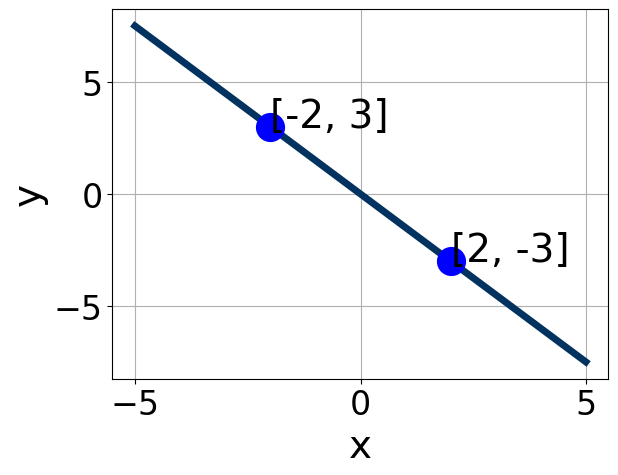
\includegraphics[width=0.5\textwidth]{../Figures/linearGraphToStandardC.png}
\end{center}
\begin{enumerate}[label=\Alph*.]
\item \( A \in [2, 8], \hspace{3mm} B \in [-4.2, -1.5], \text{ and } \hspace{3mm} C \in [8.4, 9.3] \)
\item \( A \in [-5, -2], \hspace{3mm} B \in [2.5, 5.1], \text{ and } \hspace{3mm} C \in [-9.1, -8.1] \)
\item \( A \in [-3.67, 1.33], \hspace{3mm} B \in [-0.9, 1.8], \text{ and } \hspace{3mm} C \in [-4.4, -1.4] \)
\item \( A \in [2, 8], \hspace{3mm} B \in [2.5, 5.1], \text{ and } \hspace{3mm} C \in [-9.1, -8.1] \)
\item \( A \in [-3.67, 1.33], \hspace{3mm} B \in [-2.8, -0.4], \text{ and } \hspace{3mm} C \in [2.2, 3.7] \)

\end{enumerate} }
\litem{
Find the equation of the line described below. Write the linear equation as $ y=mx+b $ and choose the intervals that contain $m$ and $b$.\[ \text{Parallel to } 3 x + 4 y = 4 \text{ and passing through the point } (7, 4). \]\begin{enumerate}[label=\Alph*.]
\item \( m \in [-0.96, -0.49] \hspace*{3mm} b \in [-10.8, -8] \)
\item \( m \in [0.65, 0.87] \hspace*{3mm} b \in [-1.9, 0.4] \)
\item \( m \in [-1.77, -0.82] \hspace*{3mm} b \in [8.7, 11.3] \)
\item \( m \in [-0.96, -0.49] \hspace*{3mm} b \in [8.7, 11.3] \)
\item \( m \in [-0.96, -0.49] \hspace*{3mm} b \in [-3.8, -2.7] \)

\end{enumerate} }
\litem{
First, find the equation of the line containing the two points below. Then, write the equation as $ y=mx+b $ and choose the intervals that contain $m$ and $b$.\[ (-8, -11) \text{ and } (8, 2) \]\begin{enumerate}[label=\Alph*.]
\item \( m \in [0.1, 1.6] \hspace*{3mm} b \in [-3.1, -2.69] \)
\item \( m \in [0.1, 1.6] \hspace*{3mm} b \in [-4.77, -4.28] \)
\item \( m \in [0.1, 1.6] \hspace*{3mm} b \in [-6.24, -5.26] \)
\item \( m \in [-2.6, 0] \hspace*{3mm} b \in [7.22, 9.11] \)
\item \( m \in [0.1, 1.6] \hspace*{3mm} b \in [3.65, 4.78] \)

\end{enumerate} }
\litem{
Solve the equation below. Then, choose the interval that contains the solution.\[ -4(12x + 17) = -18(2x -19) \]\begin{enumerate}[label=\Alph*.]
\item \( x \in [-12.99, -12.04] \)
\item \( x \in [-4.33, -2.85] \)
\item \( x \in [-3.51, -2.14] \)
\item \( x \in [9.16, 9.54] \)
\item \( \text{There are no real solutions.} \)

\end{enumerate} }
\litem{
Solve the linear equation below. Then, choose the interval that contains the solution.\[ \frac{4x + 9}{4} - \frac{9x -9}{7} = \frac{-3x -7}{3} \]\begin{enumerate}[label=\Alph*.]
\item \( x \in [-11.22, -5.22] \)
\item \( x \in [-2.07, 3.93] \)
\item \( x \in [-37, -30] \)
\item \( x \in [-5.62, -3.62] \)
\item \( \text{There are no real solutions.} \)

\end{enumerate} }
\litem{
Write the equation of the line in the graph below in Standard form $Ax+By=C$. Then, choose the intervals that contain $A, B, \text{ and } C$.
\begin{center}
    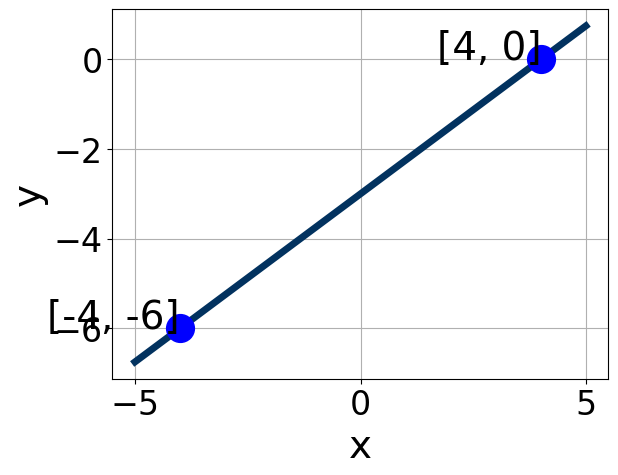
\includegraphics[width=0.5\textwidth]{../Figures/linearGraphToStandardCopyC.png}
\end{center}
\begin{enumerate}[label=\Alph*.]
\item \( A \in [2, 4], \hspace{3mm} B \in [-3.68, -2.68], \text{ and } \hspace{3mm} C \in [11, 13] \)
\item \( A \in [2, 4], \hspace{3mm} B \in [2.58, 3.41], \text{ and } \hspace{3mm} C \in [-16, -9] \)
\item \( A \in [-0.67, 0.33], \hspace{3mm} B \in [-0.49, 1.59], \text{ and } \hspace{3mm} C \in [-5, -2] \)
\item \( A \in [-0.67, 0.33], \hspace{3mm} B \in [-1.23, -0.63], \text{ and } \hspace{3mm} C \in [3, 7] \)
\item \( A \in [-8, -1], \hspace{3mm} B \in [2.58, 3.41], \text{ and } \hspace{3mm} C \in [-16, -9] \)

\end{enumerate} }
\litem{
Find the equation of the line described below. Write the linear equation as $ y=mx+b $ and choose the intervals that contain $m$ and $b$.\[ \text{Perpendicular to } 4 x + 9 y = 11 \text{ and passing through the point } (-3, 4). \]\begin{enumerate}[label=\Alph*.]
\item \( m \in [-1.7, 1] \hspace*{3mm} b \in [7.75, 13.75] \)
\item \( m \in [-3.1, -1.7] \hspace*{3mm} b \in [-2.75, 1.25] \)
\item \( m \in [1.1, 6] \hspace*{3mm} b \in [7.75, 13.75] \)
\item \( m \in [1.1, 6] \hspace*{3mm} b \in [6, 10] \)
\item \( m \in [1.1, 6] \hspace*{3mm} b \in [-10.75, -9.75] \)

\end{enumerate} }
\litem{
First, find the equation of the line containing the two points below. Then, write the equation as $ y=mx+b $ and choose the intervals that contain $m$ and $b$.\[ (8, -9) \text{ and } (-8, -10) \]\begin{enumerate}[label=\Alph*.]
\item \( m \in [0.02, 0.45] \hspace*{3mm} b \in [-4.08, -1.06] \)
\item \( m \in [0.02, 0.45] \hspace*{3mm} b \in [-10.15, -9.23] \)
\item \( m \in [0.02, 0.45] \hspace*{3mm} b \in [8.54, 10.47] \)
\item \( m \in [0.02, 0.45] \hspace*{3mm} b \in [-18.25, -15.24] \)
\item \( m \in [-0.98, 0.04] \hspace*{3mm} b \in [-10.83, -9.77] \)

\end{enumerate} }
\litem{
Solve the equation below. Then, choose the interval that contains the solution.\[ -10(8x + 15) = -16(-7x -13) \]\begin{enumerate}[label=\Alph*.]
\item \( x \in [-2, -0.1] \)
\item \( x \in [-8.8, -6.5] \)
\item \( x \in [-4, -2.6] \)
\item \( x \in [0.4, 2.7] \)
\item \( \text{There are no real solutions.} \)

\end{enumerate} }

\litem{
Solve the linear equation below. Then, choose the interval that contains the solution.\[ \frac{-3x -7}{4} - \frac{-6x -4}{7} = \frac{-5x + 8}{8} \]\begin{enumerate}[label=\Alph*.]
\item \( x \in [4.1, 5.4] \)
\item \( x \in [14.7, 17.1] \)
\item \( x \in [-0.6, 0.4] \)
\item \( x \in [1.9, 3.2] \)
\item \( \text{There are no real solutions.} \)

\end{enumerate} }
\end{enumerate}

\end{document}